\section{Proposed method: a learned warm start for phase-fixed WGS}\label{sec:proposed-method}

\subsection{Idea}\label{sec:idea}

Phase-fixed WGS~\cite{kim2019} starts from the superposition hologram of random trap phases, whose field at the traps has random phases that the first iterations must organize. The idea of the proposed method is to replace those random phases by phases that a network predicts from the geometry of the trap set, so that the first
field the iteration sees is already close to the phase pattern it would converge to. Two properties make the idea attractive on paper. First, the network is only a start: whatever it predicts, the iteration that follows is the unchanged phase-fixed WGS, so the accuracy it reaches in the limit of many iterations is that of the published method, and a bad prediction costs iterations and nothing else. Second, the iteration is
self-correcting, so the network does not need to be precise: a coarse prediction of the phase law of the array (the quadratic and periodic phase patterns that regular arrays converge to) may be enough to save iterations. The expected benefit is therefore bounded by the number of iterations the random start wastes before the field organizes. Whether that number is large is the empirical question the paper answers.

Figure~\ref{fig:method} shows the pipeline: the trap list goes through the network, the predicted phases build the start hologram, and the unchanged iteration runs from it; the weights of the iteration are not an output of the network.

\begin{figure}[t]
\centering
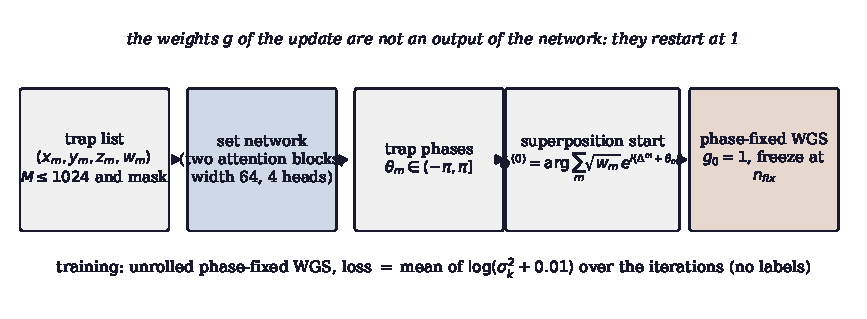
\includegraphics[width=\textwidth]{fig-method.pdf}
\caption{The learned warm start: a trap list of at most 1024 traps with a mask enters a permutation-equivariant set network that predicts one phase per trap; the superposition hologram built from those phases starts phase-fixed WGS, whose weights restart at one; training minimizes the log spread along an unrolled copy of the iteration, without labels.}
\label{fig:method}
\end{figure}

\subsection{The start hologram}\label{sec:start}

Given predicted phases $\theta_m$, the SLM start is the superposition of the single-trap holograms with those phases, the form of the SR hologram of~\cite{dileonardo} with learned instead of random phases:
\begin{equation}
\phi^{(0)}_j=\arg\sum_{m=1}^{M}a_m\,e^{\,i(\Delta_j^m+\theta_m)},\qquad a_m=\sqrt{w_m}.
\label{eq:start}
\end{equation}
This is the back-projection of the coefficients $a_me^{i\theta_m}$ of Section~\ref{sec:forward}, and it is the same operation the random start performs with $\theta_m$ drawn from the portable random generator of the engine. The start field is $V^{(0)}_m=V_m(\phi^{(0)})$ from Eq.~\eqref{eq:forward}. When the traps are well separated
the cross terms between traps are small and $\arg V^{(0)}_m\approx\theta_m$, so $\theta_m$ is, to a first approximation, the phase the iteration sees at trap $m$ in its first step. When the traps are dense the cross terms are not small, and $\arg V^{(0)}_m$ differs from $\theta_m$; this is the case of every geometry in the held-out set (at least 40 traps).

The start hologram is the only place where the network output meets the engine, and its form was chosen so that a network that predicts the right phases reproduces exactly what a converged run would hold: the phases of the converged field at the traps, back-projected with the target amplitudes. The same function builds the oracle start of Section~\ref{sec:oracle-design}, with the phases of a converged run in place of the network phases, so that the two starts differ only in where the phases come from and the comparison is not confounded by a different construction of the hologram.

\subsection{The iteration the start enters}\label{sec:m07}

Phase-fixed WGS keeps one weight $g_{k,m}$ per trap and one focal phase $\psi_{k,m}$ per trap. With $B_{k}(m)=|V^{(k)}_m|/a_m$ the trap amplitude relative to its target, the iteration for $k\ge1$ is
\begin{align}
g_{1,m}&=1,\qquad g_{k,m}=g_{k-1,m}\,\frac{\langle B_{k-1}\rangle}{B_{k-1}(m)}\quad(k\ge2),\label{eq:weights}\\
\psi_{k,m}&=\arg V^{(k-1)}_m\ \ (k\le\nfix),\qquad \psi_{k,m}=\psi_{\nfix,m}\ \ (k>\nfix),\label{eq:freeze}\\
\phi^{(k)}_j&=\arg\sum_{m=1}^{M}g_{k,m}\,a_m\,e^{\,i(\psi_{k,m}+\Delta_j^m)},\label{eq:update}
\end{align}
where $\langle\cdot\rangle$ is the mean over the traps and $\nfix$ the freeze index; the engine default of the product is $\nfix=12$ after Kim et al.~\cite{kim2019}. The weights update multiplicatively and carry the memory of all earlier corrections; the focal phase follows the field for the first $\nfix$ iterations and is then fixed, which removes the focal-phase perturbation that
re-imposing the laser amplitude at the SLM would otherwise introduce. The start enters in one place only: the field $V^{(0)}$ of Eq.~\eqref{eq:start}, which gives the phases $\psi_{1}=\arg V^{(0)}$ of the first iteration. The weights restart at one whatever the start is. The relative amplitude $B_k$ is the field amplitude $|V_m|$ divided by the target amplitude $a_m$, as in weighted GS~\cite{dileonardo}. This is the structural fact on which the theory of Section~\ref{sec:theory} rests: a warm start can only change the iteration through the phases of the first $\nfix$
steps.

\subsection{The network}\label{sec:network}

The network is a permutation-equivariant set transformer over the trap list (Set Transformer~\cite{settransformer}, Deep Sets~\cite{deepsets}). Each trap $m$ is described by its position in focal bins $(\hat x_m,\hat y_m)=(x_m,y_m)/128$, its depth in Rayleigh ranges $\hat z_m=z_m/(4z_{\mathrm R})$ and its weight, and receives a vector of $29$ features: the normalized coordinates, $\hat z_m$, $w_m-1$, $\varrho_m^2=\hat x_m^2+\hat y_m^2$, and Fourier features of the position at six octaves~\cite{fourierfeatures},
\begin{equation}
\mathbf f_m=\big[\hat x_m,\hat y_m,\hat z_m,w_m-1,\varrho_m^2,\ \sin(\pi\nu\hat x_m),\cos(\pi\nu\hat x_m),\sin(\pi\nu\hat y_m),\cos(\pi\nu\hat y_m)\big]_{\nu\in\{1,2,4,8,16,32\}}.
\label{eq:features}
\end{equation}
Two layers embed $\mathbf f_m$ to width $d=64$. Two blocks of attention follow, each with $4$ heads of width $16$, a residual connection, and a feed-forward layer of width $128$, with the padded traps removed by an additive bias of $-10^{4}$ on the attention logits:
\begin{equation}
\mathbf h\leftarrow\mathbf h+W_o\,\mathrm{softmax}\!\Big(\frac{QK^{\top}}{\sqrt{d_h}}+\mathbf b\Big)V,\qquad \mathbf h\leftarrow\mathbf h+W_2\,\mathrm{ReLU}(W_1\mathbf h),\qquad b_{jm}=-10^4\,(1-\mathrm{mask}_m),
\label{eq:attention}
\end{equation}
where $Q,K,V$ are linear maps of $\mathbf h$ and $d_h=16$; the output projections $W_o$ and $W_2$ start at zero so that the untrained network is the embedding alone. No layer normalization is used, so that the exported graph contains only operators that a browser inference runtime provides. With $\bar{\mathbf h}$ the mean of $\mathbf h$ over the valid traps, the predicted phase of trap $m$ is
\begin{equation}
\theta_m=\mathrm{wrap}\Big(\mathrm{MLP}\big([\mathbf h_m,\bar{\mathbf h}]\big)+\big(c_0+20\,\mathbf w_c^{\top}\bar{\mathbf h}\big)\,\varrho_m^2\Big),\qquad \mathrm{wrap}(t)=\operatorname{atan2}(\sin t,\cos t),
\label{eq:output}
\end{equation}
where the second term is a set-dependent quadratic (Fresnel-like) phase law with a learned scalar $c_0$ (initialized at $80$) and a learned vector $\mathbf w_c$; it lets the network write the chirp that a regular array's converged phases follow without having to represent hundreds of radians with an MLP. The network has $\nParams$ parameters and its ONNX export holds $\onnxBytes$ bytes. The value of $c_0$ after training is the initial one to
within a fraction of a percent, so the learned part is the correction on top of the chirp.

\subsection{Training without labels}\label{sec:training}

Converged WGS phases are not unique: the global phase is free and the many fixed points of the iteration give different phases for the same geometry, so a regression onto converged phases would have an ambiguous target. We train instead through the iteration. A differentiable copy of Eqs.~\eqref{eq:weights}--\eqref{eq:update} (separable point-trap form in single precision, checked against the engine's phase-fixed WGS in the repository's tests) is
unrolled for $K=10$ iterations from the start of Eq.~\eqref{eq:start}, and the loss is the weighted mean of the log of the squared spread:
\begin{equation}
\mathcal L(\vartheta)=\frac{1}{\sum_{k=0}^{K}\omega_k}\sum_{k=0}^{K}\omega_k\ \mathbb E_{\mathcal T\sim\mathcal D}\Big[\log\big(\relstd_k^2+0.01\big)\Big],\qquad \omega_0=0.3,\ \omega_{k\ge1}=1,
\label{eq:loss}
\end{equation}
with $\relstd_k$ the spread (in percent) after unrolled iteration $k$ and $\relstd_0$ that of the start. The constant $0.01$ saturates the loss below a spread of 0.1 percent, so that the network is not rewarded for precision the iteration reaches by itself; the log compresses the large spreads of the first iterations. The unrolled iteration uses the freeze index $\nfix=3$, chosen because an earlier trial at
$\nfix=12$ with 14 unrolled iterations produced a start that reached about the random level. The global phase is invariant by construction because the loss reads intensities only. The trap sets are drawn on the fly from seeded generators: square and hexagonal lattices, rings with an optional concentric ring, random sets with a minimum spacing, stacks of two to four planes and random three-dimensional sets, with the proportions
$0.25$, $0.15$, $0.15$, $0.2$, $0.15$, $0.1$, optional position jitter and random weights in $[0.5,2]$ for 30 percent of the sets; sets of fewer than 40 traps are discarded with probability $0.6$ because a sparse array reaches 1 percent at the first iteration from any start. The generators contain no quasi-periodic family, so the benchmark geometry of that kind is unseen.

\subsection{Algorithms and parameters}\label{sec:algorithm}

Algorithm~\ref{alg:warm} is the method as run by the engine; Algorithm~\ref{alg:train} is the offline training. The inference algorithm has two branches that matter for the interpretation of every measurement below: when a network is released the phases come from it, and when none is released the phases are drawn from the seeded generator, so that the same function answers in both cases and the baseline is not a different code path. The training algorithm sees only trap sets and the differentiable iteration; it never reads a held-out geometry and never reads a converged phase, which is what makes it unsupervised in the sense of the problem statement.

\begin{algorithm}[t]
\caption{Learned warm start for phase-fixed WGS (inference and run).}\label{alg:warm}
\begin{algorithmic}[1]
\Require trap set $\mathcal T=\{(x_m,y_m,z_m,w_m)\}$, network $g_\vartheta$ (or none), freeze index $\nfix$, budget $K_{\max}$, seed
\Ensure SLM phase $\phi^{(K)}$ and the history $\relstd(\phi^{(k)})$
\State convert $\mathcal T$ to bins and Rayleigh ranges, pad to $1024$ traps with a mask
\If{a network is released} $\theta\gets g_\vartheta(\mathcal T)$ \Else{} $\theta_m\sim U[0,2\pi)$ from the seeded generator \EndIf
\State $\phi^{(0)}\gets\arg\sum_ma_me^{i(\Delta^m+\theta_m)}$ \Comment{Eq.~\eqref{eq:start}}
\State $V^{(0)}\gets$ project$(\phi^{(0)})$;\quad $g_1\gets\mathbf 1$
\For{$k=1,\dots,K_{\max}$}
  \If{$k\ge2$} $g_k\gets g_{k-1}\langle B_{k-1}\rangle/B_{k-1}$ \EndIf \Comment{Eq.~\eqref{eq:weights}}
  \State $\psi_k\gets\arg V^{(k-1)}$ if $k\le\nfix$, else $\psi_{\nfix}$ \Comment{Eq.~\eqref{eq:freeze}}
  \State $\phi^{(k)}\gets\arg\sum_mg_{k,m}a_me^{i(\psi_{k,m}+\Delta^m)}$;\quad $V^{(k)}\gets$ project$(\phi^{(k)})$ \Comment{Eq.~\eqref{eq:update}}
\EndFor
\State \Return $\phi^{(K_{\max})}$ and the history of $\relstd$, $\eta$, $u$
\end{algorithmic}
\end{algorithm}

\begin{algorithm}[t]
\caption{Unsupervised training of the warm-start network through the unrolled iteration.}\label{alg:train}
\begin{algorithmic}[1]
\Require generator of trap sets $\mathcal D$ with a seed, steps $T$, batch $B$, unroll $K$, freeze index $\nfix$
\State initialize $\vartheta$ from the initialization seed; AdamW with a warm-up and a cosine schedule
\For{$t=1,\dots,T$}
  \State draw $B$ trap sets, pad and mask;\quad $\theta\gets g_\vartheta(\mathcal T)$
  \State run the unrolled iteration for $K$ steps from the start of Eq.~\eqref{eq:start}, recording $\relstd_0,\dots,\relstd_K$
  \State $\mathcal L\gets$ Eq.~\eqref{eq:loss};\quad clip the gradient norm to $1$;\quad update $\vartheta$
\EndFor
\State \Return $\vartheta$ \Comment{evaluated on held-out geometries before any release}
\end{algorithmic}
\end{algorithm}

Table~\ref{tab:params} lists every parameter of the method with its value and where the value comes from. Values that are choices of the product, not of a source, are marked as such. The architecture was sized to the limit the product sets for a model that a browser must download and run, at most 1 MB as an exported graph, and the training budget to what a single laptop GPU delivers in under two hours; neither was tuned against the held-out set, which training never reads. The freeze index of the training unroll, $\nfix=3$, is the one parameter that departs from the published default, and it is the parameter that the ablation of Section~\ref{sec:ablation} isolates.

\begin{table}[t]
\centering\small
\begin{tabular}{@{}lll@{}}
\toprule
Parameter & Value & Origin \\
\midrule
width $d$, layers, heads, feed-forward & 64, 2, 4, 128 & choice of the product, sized to stay under 1 MB \\
Fourier octaves $\nu$ & 1, 2, 4, 8, 16, 32 & choice of the product after~\cite{fourierfeatures} \\
maximum number of traps & 1024 & contract of the model slot \\
unroll $K$, freeze index in training & 10, 3 & choice of the product (Section~\ref{sec:training}) \\
loss constants $0.01$, $\omega_0$ & 0.01, 0.3 & choice of the product \\
steps, batch, peak learning rate & 6000, 8, $8\times10^{-4}$ & choice of the product (AdamW~\cite{adamw}, decay $10^{-5}$) \\
data seed, initialization seed & 20261101, 7 & recorded in the training configuration \\
freeze index of the engine default $\nfix$ & 12 & Kim et al.~\cite{kim2019} \\
iteration budget $K_{\max}$ & \budget & evaluation protocol (Section~\ref{sec:design}) \\
\bottomrule
\end{tabular}
\caption{Parameters of the learned warm start and of the iteration it feeds, with their origin; the network and training values are those of the trained candidate whose configuration is recorded with its checkpoint.}
\label{tab:params}
\end{table}

\subsection{Complexity and implementation}\label{sec:complexity}

The attention of a block over $M$ traps costs $M^2d$ multiply-adds for $QK^\top$ and the same for the weighted sum, that is $2M^2d$ per block, so inference is $O(LM^2d)$ for $L$ blocks, plus $O(Md^2)$ for the linear layers; the full attention is quadratic in the number of traps, not linear. Counting the multiply-adds of the attention products and of one iteration of the point form of phase-fixed WGS (a projection and a back-projection, each a separable product of $N^2M$ terms),
\begin{equation}
C_{\mathrm{net}}\approx 2\,L\,M^{2}d,\qquad C_{\mathrm{iter}}\approx 2\,N^{2}M,
\label{eq:cost}
\end{equation}
which at the maximum of $M=1024$ traps, $L=2$, $d=64$ and $N=256$ give about $2.7\times10^{8}$ and $1.3\times10^{8}$ multiply-adds, so by operation count the network pass at the largest array is of the order of two iterations of the method it is meant to shorten. The start hologram of Eq.~\eqref{eq:start} costs one back-projection, as one iteration does. Training is offline and local, on one GPU, never in the continuous
integration of the product.

The method is implemented in the engine of the product as the module \texttt{methods/learned/b3\_warm\_start.py} (the method), \texttt{learned/nets.py} (the network), \texttt{learned/torch\_forward.py} (the differentiable iteration), \texttt{learned/training.py} (Algorithm~\ref{alg:train}) and \texttt{learned/heldout.py} and \texttt{learned/evaluation.py} (the held-out sets and the evaluation of Section~\ref{sec:design}). With no released network, the module answers with the iteration from its own random start and marks the result as a baseline, so that
a missing model is never mistaken for a learned one.
